\documentclass[tikz,border=5pt]{standalone}
\usepackage{luatexja}
\usepackage[hiragino-pron]{luatexja-preset}
\usepackage{amsmath,amssymb}
\usetikzlibrary{arrows.meta,patterns,decorations.pathreplacing}

\begin{document}
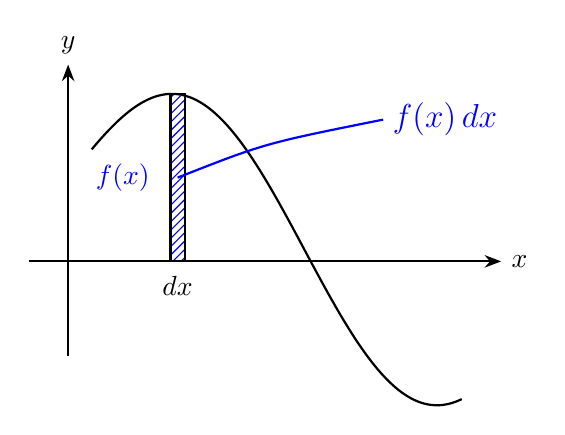
\begin{tikzpicture}

% Axes
\draw[-{Stealth[length=6pt]}, thick] (-0.5,0) -- (5.5,0) node[right] {$x$};
\draw[-{Stealth[length=6pt]}, thick] (0,-1.2) -- (0,2.5) node[above] {$y$};

% f(x) curve
\draw[thick, domain=0.3:5, samples=80, smooth]
  plot (\x, {1.5*sin(60*\x) - 0.3*(\x-2.5) + 0.3});

% Thin strip at x ~ 1.3
\pgfmathsetmacro{\xstrip}{1.3}
\pgfmathsetmacro{\dxw}{0.18}
\pgfmathsetmacro{\fval}{1.5*sin(60*\xstrip) - 0.3*(\xstrip-2.5) + 0.3}

% Fill strip
\fill[pattern=north east lines, pattern color=blue]
  (\xstrip,0) rectangle (\xstrip+\dxw,\fval);
\draw[thick] (\xstrip,0) rectangle (\xstrip+\dxw,\fval);

% f(x) height label
\node[left=4pt, blue] at (\xstrip,\fval/2) {$f(x)$};

% Label dx
\node[below=2pt] at (\xstrip+\dxw/2,0) {$dx$};

% Label f(x)dx with line from strip
\node[blue, right] (fxdx) at (4,1.8) {\large $f(x)\,dx$};
\draw[blue, thick] (\xstrip+\dxw/2,\fval/2) .. controls (2.5,1.5) .. (fxdx.west);


\end{tikzpicture}
\end{document}
